\documentclass{standalone}

\usepackage{amsmath,amssymb}

\usepackage{tikz}
\usetikzlibrary{quantikz}
\usetikzlibrary{decorations.pathmorphing}
\usetikzlibrary{shapes.arrows}
\usetikzlibrary{calc,math}

\usepackage{physics}


\begin{document}

\tikzset{every picture/.style={line width=0.75pt}} %set default line width to 0.75pt        

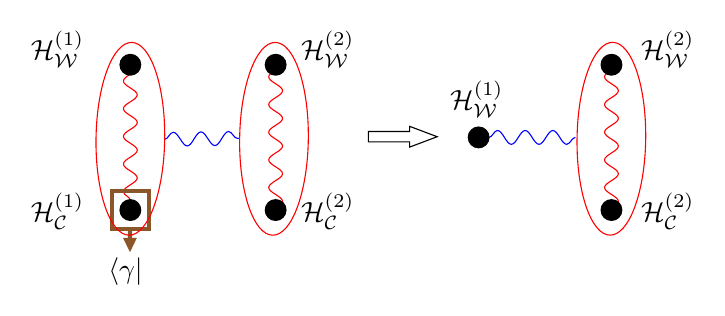
\begin{tikzpicture}[x=0.75pt,y=0.75pt,yscale=-1,xscale=1]
%uncomment if require: \path (0,232); %set diagram left start at 0, and has height of 232

%Straight Lines [id:da2698248251783375] 
\draw [draw=red, decorate, decoration=snake] (186,62) -- (186,135) ;
%Straight Lines [id:da9636019489378673] 
\draw  [draw=red, decorate, decoration=snake]  (256,60) -- (256,135) ;
%Straight Lines [id:da7979765257489624] 
\draw [draw=blue, decorate, decoration=snake] (202.54,100.92) -- (238.66,100.44) ;
%Shape: Circle [id:dp17171950821270499] 
\draw  [fill={rgb, 255:red, 0; green, 0; blue, 0 }  ,fill opacity=1 ] (181,65) .. controls (181,62.24) and (183.24,60) .. (186,60) .. controls (188.76,60) and (191,62.24) .. (191,65) .. controls (191,67.76) and (188.76,70) .. (186,70) .. controls (183.24,70) and (181,67.76) .. (181,65) -- cycle ;
%Shape: Circle [id:dp7539614365582425] 
\draw  [fill={rgb, 255:red, 0; green, 0; blue, 0 }  ,fill opacity=1 ] (181,135) .. controls (181,132.24) and (183.24,130) .. (186,130) .. controls (188.76,130) and (191,132.24) .. (191,135) .. controls (191,137.76) and (188.76,140) .. (186,140) .. controls (183.24,140) and (181,137.76) .. (181,135) -- cycle ;
%Shape: Circle [id:dp5479550400453568] 
\draw  [fill={rgb, 255:red, 0; green, 0; blue, 0 }  ,fill opacity=1 ] (251,65) .. controls (251,62.24) and (253.24,60) .. (256,60) .. controls (258.76,60) and (261,62.24) .. (261,65) .. controls (261,67.76) and (258.76,70) .. (256,70) .. controls (253.24,70) and (251,67.76) .. (251,65) -- cycle ;
%Shape: Circle [id:dp4938703436561742] 
\draw  [fill={rgb, 255:red, 0; green, 0; blue, 0 }  ,fill opacity=1 ] (251,135) .. controls (251,132.24) and (253.24,130) .. (256,130) .. controls (258.76,130) and (261,132.24) .. (261,135) .. controls (261,137.76) and (258.76,140) .. (256,140) .. controls (253.24,140) and (251,137.76) .. (251,135) -- cycle ;
%Shape: Rectangle [id:dp24725342060756206] 
\draw  [color={rgb, 255:red, 139; green, 87; blue, 42 }  ,draw opacity=1 ][line width=1.5]  (177,126) -- (195,126) -- (195,144) -- (177,144) -- cycle ;
%Straight Lines [id:da7435547473684463] 
\draw [color={rgb, 255:red, 139; green, 87; blue, 42 }  ,draw opacity=1 ][line width=1.5]    (185.8,143.8) -- (185.82,151.33) ;
\draw [shift={(185.83,155.33)}, rotate = 269.83] [fill={rgb, 255:red, 139; green, 87; blue, 42 }  ,fill opacity=1 ][line width=0.08]  [draw opacity=0] (6.97,-3.35) -- (0,0) -- (6.97,3.35) -- cycle    ;
%Right Arrow [id:dp5596697397183885] 
\draw   (300.67,97.17) -- (320.57,97.17) -- (320.57,94.67) -- (333.83,99.67) -- (320.57,104.67) -- (320.57,102.17) -- (300.67,102.17) -- cycle ;
%Straight Lines [id:da1417261779211143] 
\draw [draw=blue, decorate, decoration=snake] (400.4,100) -- (353.8,100) ;
%Straight Lines [id:da8022192144372267] 
\draw [draw=red, decorate, decoration=snake] (417.8,60) -- (417.8,135) ;
%Shape: Circle [id:dp9476748423291472] 
\draw  [fill={rgb, 255:red, 0; green, 0; blue, 0 }  ,fill opacity=1 ] (348.8,100) .. controls (348.8,97.24) and (351.04,95) .. (353.8,95) .. controls (356.56,95) and (358.8,97.24) .. (358.8,100) .. controls (358.8,102.76) and (356.56,105) .. (353.8,105) .. controls (351.04,105) and (348.8,102.76) .. (348.8,100) -- cycle ;
%Shape: Circle [id:dp9505056317553204] 
\draw  [fill={rgb, 255:red, 0; green, 0; blue, 0 }  ,fill opacity=1 ] (412.8,65) .. controls (412.8,62.24) and (415.04,60) .. (417.8,60) .. controls (420.56,60) and (422.8,62.24) .. (422.8,65) .. controls (422.8,67.76) and (420.56,70) .. (417.8,70) .. controls (415.04,70) and (412.8,67.76) .. (412.8,65) -- cycle ;
%Shape: Circle [id:dp730831673390409] 
\draw  [fill={rgb, 255:red, 0; green, 0; blue, 0 }  ,fill opacity=1 ] (412.8,135) .. controls (412.8,132.24) and (415.04,130) .. (417.8,130) .. controls (420.56,130) and (422.8,132.24) .. (422.8,135) .. controls (422.8,137.76) and (420.56,140) .. (417.8,140) .. controls (415.04,140) and (412.8,137.76) .. (412.8,135) -- cycle ;
%Shape: Ellipse [id:dp4600391404472841] 
\draw [color=red] (401.22,100.41) .. controls (401.58,74.76) and (409.29,54.07) .. (418.42,54.2) .. controls (427.55,54.33) and (434.66,75.23) .. (434.29,100.88) .. controls (433.93,126.53) and (426.22,147.22) .. (417.09,147.09) .. controls (407.96,146.96) and (400.85,126.06) .. (401.22,100.41) -- cycle ;
%Shape: Ellipse [id:dp7196405870617228] 
\draw [color=red] (169.46,100.44) .. controls (169.83,74.79) and (177.53,54.11) .. (186.66,54.24) .. controls (195.8,54.37) and (202.9,75.27) .. (202.54,100.92) .. controls (202.17,126.57) and (194.47,147.26) .. (185.34,147.12) .. controls (176.2,146.99) and (169.1,126.09) .. (169.46,100.44) -- cycle ;
%Shape: Ellipse [id:dp33388546166070765] 
\draw [color=red] (238.66,100.44) .. controls (239.03,74.79) and (246.73,54.11) .. (255.86,54.24) .. controls (265,54.37) and (272.1,75.27) .. (271.74,100.92) .. controls (271.37,126.57) and (263.67,147.26) .. (254.54,147.12) .. controls (245.4,146.99) and (238.3,126.09) .. (238.66,100.44) -- cycle ;

% Text Node
\draw (136.8,47.4) node [anchor=north west][inner sep=0.75pt]    {$\mathcal{H}^{( 1)}_{\mathcal{W}}$};
% Text Node
\draw (267,47.4) node [anchor=north west][inner sep=0.75pt]    {$\mathcal{H}^{( 2)}_{\mathcal{W}}$};
% Text Node
\draw (136.8,125.4) node [anchor=north west][inner sep=0.75pt]    {$\mathcal{H}^{( 1)}_{\mathcal{C}}$};
% Text Node
\draw (267,125.4) node [anchor=north west][inner sep=0.75pt]    {$\mathcal{H}^{( 2)}_{\mathcal{C}}$};
% Text Node
\draw (174.13,156.73) node [anchor=north west][inner sep=0.75pt]    {$\langle \gamma |$};
% Text Node
\draw (338.8,71.4) node [anchor=north west][inner sep=0.75pt]    {$\mathcal{H}^{( 1)}_{\mathcal{W}}$};
% Text Node
\draw (430.8,47.4) node [anchor=north west][inner sep=0.75pt]    {$\mathcal{H}^{( 2)}_{\mathcal{W}}$};
% Text Node
\draw (430.8,125.4) node [anchor=north west][inner sep=0.75pt]    {$\mathcal{H}^{( 2)}_{\mathcal{C}}$};


\end{tikzpicture}

\end{document}
